%!TEX program = xelatex
\documentclass[dvipsnames, svgnames,a4paper,11pt]{article}
% ----------------------------------------------------
%   中山大学物理与天文学院本科实验报告模板
%   作者:Huanyu Shi,2019级
%   知乎:https://www.zhihu.com/people/za-ran-zhu-fu-liu-xing
%   Github:https://github.com/huanyushi/SYSU-SPA-Labreport-Template
%   Last update : 2023.4.10
% ----------------------------------------------------

% ----------------------------------------------------- 
%	加边框的命令
%	参考:https://tex.stackexchange.com/questions/531559/how-to-add-the-page-border-for-first-two-pages-in-latex
\usepackage{tikz}
\usetikzlibrary{calc}
\usepackage{eso-pic}
\AddToShipoutPictureBG{%
\begin{tikzpicture}[overlay,remember picture]
\draw[line width=0.6pt] % 边框粗细
    ($ (current page.north west) + (0.6cm,-0.6cm) $)
    rectangle
    ($ (current page.south east) + (-0.6cm,0.6cm) $); % 边框位置
\end{tikzpicture}}


\usepackage{xcolor}
\definecolor{c1}{HTML}{2752C9} % 目录颜色
\definecolor{c2}{RGB}{190,20,83} % 引用颜色

\usepackage{ctex}
\usepackage[top=28mm,bottom=28mm,left=15mm,right=15mm]{geometry}
\usepackage{hyperref} 
\hypersetup{
	colorlinks,
	linktoc = section, % 超链接位置,选项有section, page, all
	linkcolor = c1, % linkcolor 目录颜色
	citecolor = c1  % citecolor 引用颜色
}
\usepackage{amsmath,enumerate,multirow,float}
\usepackage{tabularx}
\usepackage{tabu}
\usepackage{subfig}
\usepackage{fancyhdr}
\usepackage{graphicx}
\usepackage{wrapfig}  
\usepackage{physics}
\usepackage{appendix}
\usepackage{amsfonts}

%
\usepackage{tcolorbox}
\tcbuselibrary{skins,breakable}
\newtcolorbox{tbox}[2][]{
    colframe=black!70!,
    breakable,
    enhanced,
	boxrule =0.5pt,
    title = {#2},
    fonttitle = \large\kaishu\bfseries,
	drop fuzzy shadow,
    #1
}
\newtcolorbox[auto counter,number within=section]{question}[1][]{
  top=2pt,bottom=2pt,arc=1mm,
  boxrule=0.5pt,
%   frame hidden,
  breakable,
  enhanced, %跨页后不会显示下边框
  coltitle=c1!80!gray,
  colframe=c1,
  colback=c1!3!white,
  drop fuzzy shadow,
  title={思考题~\thetcbcounter:\quad},
  fonttitle=\bfseries,
  attach title to upper,
  #1
}

% ---------------------------------------------------------------------
%	利用cleveref改变引用格式,\cref是引用命令
\usepackage{cleveref}
\crefformat{figure}{#2{\textcolor{c2}{图 #1}}#3} % 图片的引用格式
\crefformat{equation}{#2{(\textcolor{c2}{#1})}#3} % 公式的引用格式
\crefformat{table}{#2{\textcolor{c2}{表 #1}}#3} % 表格的引用格式


% ---------------------------------------------------------------------
%	页眉页脚设置
\fancypagestyle{plain}{\pagestyle{fancy}}
\pagestyle{fancy}
\lhead{\kaishu 中山大学物理与天文学院近代物理实验\uppercase\expandafter{\romannumeral1}} % 左边页眉,学院 + 课程
\rhead{\kaishu D4-1 \quad 电子自旋共振实验} % 右边页眉,实验报告标题
\cfoot{\thepage} % 页脚,中间添加页码


% ---------------------------------------------------------------------
%	对目录、章节标题的设置
\renewcommand{\contentsname}{\centerline{\huge 目录}}
\usepackage{titlesec}
\usepackage{titletoc}
% \titleformat{章节}[形状]{格式}{标题序号}{序号与标题间距}{标题前命令}[标题后命令]
\titleformat{\section}{\centering\LARGE\songti}{}{1em}{}

% ---------------------------------------------------------------------
%   listing代码环境设置
\usepackage{listings}
\lstloadlanguages{python}
\lstdefinestyle{pythonstyle}{
backgroundcolor=\color{gray!5},
language=python,
frameround=tftt,
frame=shadowbox, 
keepspaces=true,
breaklines,
columns=spaceflexible,                   
basicstyle=\ttfamily\small, % 基本文本设置,字体为teletype,大小为scriptsize
keywordstyle=[1]\color{c1}\bfseries, 
keywordstyle=[2]\color{Red!70!black},   
stringstyle=\color{Purple},       
showstringspaces=false,
commentstyle=\ttfamily\scriptsize\color{green!40!black},%注释文本设置,字体为sf,大小为smaller
tabsize=2,
morekeywords={as},
morekeywords=[2]{np, plt, sp},
numbers=left, % 代码行数
numberstyle=\it\tiny\color{gray}, % 代码行数的数字字体设置
stepnumber=1,
rulesepcolor=\color{gray!30!white}
}




% ---------------------------------------------------------------------
%	其他设置
\def\degree{${}^{\circ}$} % 角度
\graphicspath{{./images/}} % 插入图片的相对路径
\allowdisplaybreaks[4]  %允许公式跨页 % 导入模板的相关设置
\usepackage{lipsum}
\usepackage{enumitem}
\usepackage{tabularray}  %绘制表格时可以更加方便添加框线
\usepackage{titling} % 引入titling宏包
\usepackage{subcaption}

\setlist[enumerate]{label=\textup{(\arabic*)}}





% \title{热力学第二定律设计性实验}
% \pretitle{\begin{center}\LARGE\bfseries}
% \posttitle{\par\end{center}\vskip 0.5em}

% \preauthor{}
% \postauthor{}

% \author{
%     \begin{center}
%         \begin{tabular}{ll}
%             \underline{戴鹏辉} & 学号:\underline{22344016} \\
%             姓名:\underline{杨舒云} & 学号:\underline{22344020}
%         \end{tabular}
%     \end{center}
% }

% \date{}

% % 自定义命令用于插入副标题
% \newcommand{\   subtitle}[1]{%
%     \begin{center}\large#1\end{center}%
%     \vskip 1em
% }

%---------------------------------------------------------------------
%	正文
%---------------------------------------------------------------------

\begin{document}

\begin{center}
    {\Huge \textbf{热力学第二定律设计性实验}} \\
    \bigskip
    {\Large \textbf{基于热电效应的热机设计与热力学第二定律验证实验}}

\end{center}

\begin{table}[htbp]
    \centering
    \begin{tblr}{
    }
    姓名: & \underline{戴鹏辉} & 学号: & \underline{22344016} \\
    姓名: & \underline{杨舒云} & 学号: & \underline{22344020} 
    \end{tblr}
\end{table}


\clearpage
\tableofcontents
\clearpage



\section{摘要}






\section{背景介绍}

    \subsection{热力学第一定律与热力学第二定律}
        
        \begin{itemize}
            \item \textbf{热力学第一定律:}热力学第一定律,又称能量守恒定律,指出在一个孤立系统中,能量既不会凭空产生也不会凭空消失,只会从一种形式转化为另一种形式。这一定律表明了能量守恒的原理,即系统的总能量变化等于系统所吸收的热量与所做功的总和。用数学形式表示为:
            \[
            \Delta U = Q + W
            \]
            其中 $\Delta U$ 是系统内能的变化,$Q$ 系统是吸收的热量,$W$ 是外界对系统做的功。热力学第一定律奠定了热能与机械能之间的转换关系,是热机和其他能量转换装置设计的基础。
            

            \item \textbf{热力学第二定律:}热力学第二定律描述了自然界中能量转移的方向性和不可逆性,具体表述为克劳修斯表述和开尔文表述。

                \begin{itemize}
                    \item \textbf{克劳修斯表述:}
                    \begin{enumerate}
                        \item 热力学第二定律的克劳修斯表述指出,不可能将热量从低温物体自发地传递给高温物体,而不引起其他变化。
                        \item 这表明了热量传递的方向性,即热量不会自发地从冷物体流向热物体。
                    \end{enumerate}
                    
                    \item \textbf{开尔文表述:}
                    \begin{enumerate}
                        \item 另一种表述是开尔文表述,它指出不可能从单一热源吸热使之完全转化为功而不产生其他影响。
                        \item 这个表述强调了能量转化过程中不可避免的能量损耗或者其他形式的能量转移。
                    \end{enumerate}
                \end{itemize}

        
        \end{itemize}



        % \begin{itemize}
        %     \item \textbf{克劳修斯表述:}
        %         \begin{enumerate}
        %             \item 热力学第二定律的克劳修斯表述指出,不可能将热量从低温物体自发地传递给高温物体,而不引起其他变化。
                    
        %             \item 这表明了热量传递的方向性,即热量不会自发地从冷物体流向热物体。
                    
        %         \end{enumerate}
            
        %     \item \textbf{开尔文表述:}
        %         \begin{enumerate}
        %             \item 另一种表述是开尔文表述,它指出不可能从单一热源吸热使之完全转化为功而不产生其他影响。
                    
        %             \item 这个表述强调了能量转化过程中不可避免的能量损耗或者其他形式的能量转移。
                    
        %         \end{enumerate}
            

        % \end{itemize}

        % 这些表述共同揭示了热力学第二定律的普遍趋势:自然界中热量总是朝着热量分布更均匀的状态转移,不会自发地产生从低温到高温的热量流动。热力学第二定律的理论基础支持了许多热力学和工程学中的实际应用,如热机、制冷机和能量转换系统的设计与优化。在自然界和工程技术中,这一定律的应用指导了许多过程的进行和技术的发展,例如能源的有效利用和环境保护等方面。



        


    
    \subsection{热机}

        \begin{itemize}
            \item \textbf{热机的基本原理:}热机的基本工作原理基于热力学定律,特别是热力学第一定律(能量守恒定律)和第二定律(熵增原理)。简单来说,热机利用高温热源和低温热汇之间的温差,通过一定的循环过程将部分热能转化为机械能或电能,而未转化的部分热能则被低温热汇吸收。\textbf{热电发电机}则利用塞贝克效应(Seebeck Effect)将热能直接转化为电能。
            
            \item \textbf{热电发电机的优缺点:}热电发电机具有无运动部件、静音运行、模块化设计和多种热源适应性的优点,因此它具有高可靠性、低维护需求、易于集成和扩展,并能够利用太阳能、地热、废热等多种形式的热源。然而,它也存在能量转换效率较低(一般在5\%到10\%之间)和成本较高的缺点,这些限制了其大规模应用。通过材料研究和制造工艺的改进,未来有望提升效率并降低成本,使其在更多领域得到广泛应用。
            
        \end{itemize}
















\section{基本原理与实验方案}
    
    
    \subsection{基本原理}

        \begin{enumerate}
            \item \textbf{热电效应:}
            
                \begin{itemize}
                    \item Seebeck 效应:当两种不同的导体或半导体连接成回路,并且两个接头的温度不同,就会在回路中产生\textbf{电动势}
                    
                        \[
                            \mathrm{d}V=\epsilon_{AB}\mathrm{d}T
                        \]
                        其中,$\epsilon_{AB}$是温差电动势系数(又称\textbf{Seebeck系数},记为$\alpha$)。符号约定为如果在高温段电动势驱使电流由金属A流向金属B为正。
        
                        \begin{figure}[htbp]
                            \centering
                            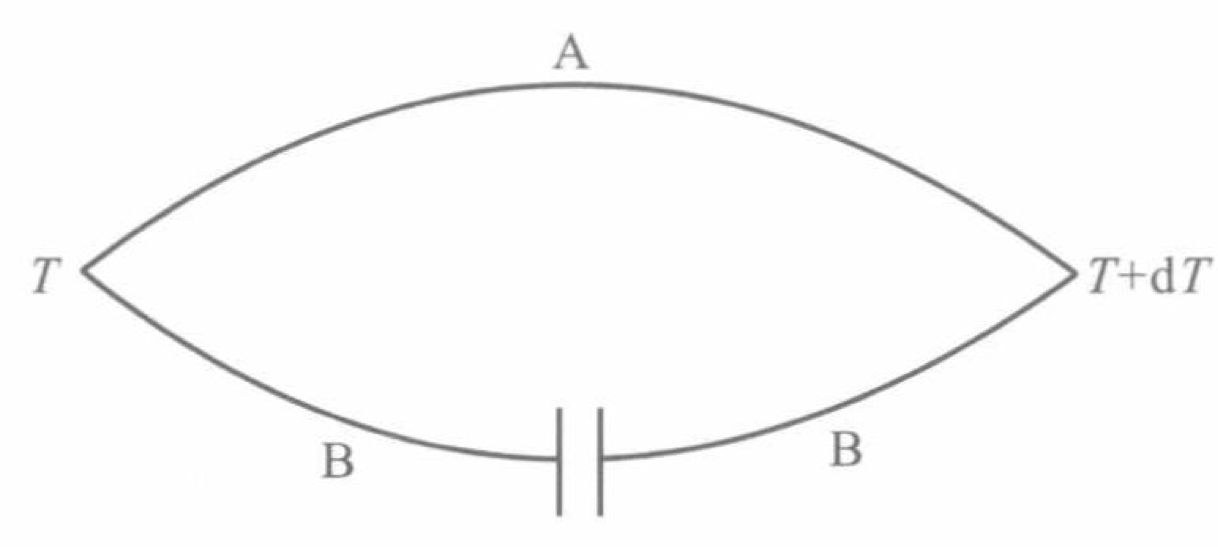
\includegraphics[width=0.45\textwidth]{SamPre_1_Gra1.jpg}
                        \end{figure}
        
                    \item Peltier效应: 当电流通过两种不同材料组成的电路时,一个接头会吸热,另一个接头会放热。
                    
                        \[
                            \textbf{J}_{q\pi}=\pi_{AB}\textbf{J}_{e}
                        \]
        
                        其中,$\textbf{J}_{q\pi}$是Peltier热流密度,$\textbf{J}_{e}$是从A到B的电流密度,$\pi_{AB}$是两种金属的Peltier系数(与温度有关)。
        
                        \begin{figure}[htbp]
                            \centering
                            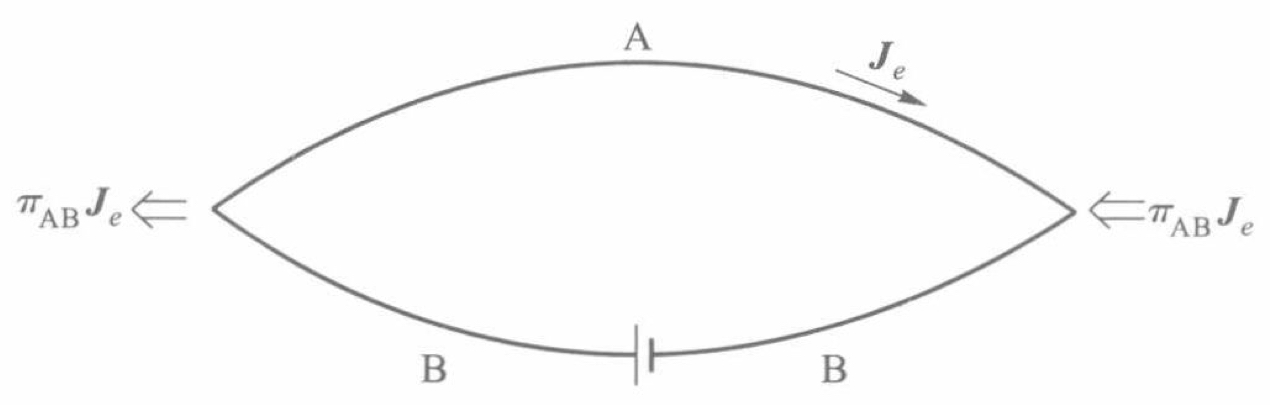
\includegraphics[width=0.5\textwidth]{SamPre_1_Gra2.jpg}
                        \end{figure}
        
        
                    
                    \item Thomson效应:在均质导体中,如果存在温度梯度,当电流通过时,会伴随着吸热或放热的现象。这对于完整的热电模型和效率分析很关键。$\dot{Q}=\mu I\cdot \nabla T$,$\mu$为Thomson系数。
        
        
                \end{itemize}




            \item \textbf{Seebeck效应电源的外输出特性:}
            

                
                \begin{itemize}
                    \item 开路电压是指没有外部负载连接时,热电发电装置两端的电压。根据Seebeck效应,开路电压与温差成正比,$V_{\text{oc}} = \alpha \Delta T$。
                    
                    \item 当热电发电装置连接到负载时,输出电压会由于内阻的存在而下降。负载电压$V_{\text{L}} = \frac{\alpha \Delta T \cdot R_{\text{L}}}{R_{\text{L}} + R_{\text{in}}}$,而输出功率是负载上消耗的功率$P_{\text{out}} = \frac{(\alpha \Delta T)^2 \cdot R_{\text{L}}}{(R_{\text{L}} + R_{\text{in}})^2}$。
                    
                    \item \textbf{当负载电阻等于内阻时},热电发电装置输出的功率达到最大$P_{\text{max}} = \frac{(\alpha \Delta T)^2}{4 R_{\text{in}}}$。				
                \end{itemize}	





            \item \textbf{PID控温:}
            

                \begin{itemize}
                    \item PID(Proportional-Integral-Derivative)控制是一种用于温度控制的经典算法,通过对误差的比例、积分和微分进行计算和调整,精确控制加热器的输出,从而实现温度的稳定控制。PID 控制器通常由三个部分组成:比例(P),积分(I),和微分(D)。
                    
                    \item PID 控温的控制量 $u(t)$ 可以表示为:$$u(t) = K_p e(t) + K_i \int_0^t e(\tau) d\tau + K_d \frac{d e(t)}{dt}$$
                    
                    \item 比例控制$P_{\text{out}} = K_p e(t)$直接与当前误差成比例,调整系统响应速度;积分控制$I_{\text{out}} = K_i \int_0^t e(\tau) d\tau$对误差进行积分,消除稳态误差,增强系统的长期精度;微分控制$D_{\text{out}} = K_d \frac{d e(t)}{dt}$对误差进行微分,预测误差变化趋势,减小超调和振荡。
                \end{itemize}	



      \end{enumerate}








    \subsection{实验方案}
    
        \begin{enumerate}
            \item 各元件性能测量
            \begin{itemize}
                \item \textbf{Seebeck效应测量}:通过改变温差并测量开路电压来研究Seebeck效应,从而确定$\alpha$;
                \item 器件内阻的测量与影响:内阻对热电转换效率有重要影响,了解并优化内阻对提高热机性能是必要的;
                \item 考虑测量电加热器的加热功率(以及其它元件性能,如Peltier效应)。
            \end{itemize}
            
            \item 搭建热机
                \begin{itemize}
                    \item \textbf{热电堆集成——电加热器与Seebeck元件,测控部分——PID控温(热端、冷端),输出电路部分(输出功率测量)。}
                \end{itemize}
            
            \item 负载与效率测量
            \begin{itemize}
                \item \textbf{加热功率测控}——电流表电压表实时测控(含于PID系统中,编写相关程序);
                \item \textbf{输出功率测控}——电流表电压表实时测控(考虑是否编程);
                \item 测量最大输出功率——改变输出电路的负载;
                \item 测量最大输出效率——改变温差与负载,优化其它部分;
                \item 探究如何测量热端的损失。
            \end{itemize}
            
            \item 热力学第二定律的展示
            \begin{itemize}
                \item \textbf{通过实验测量,展示即使是优化过的热电装置,其效率也受到卡诺效率的限制,这直接体现了热力学第二定律。}
                \item 讨论如何通过实验设计来逼近卡诺效率,包括使用最佳材料、最佳温差和最佳负载条件。
            \end{itemize}			
            
            \item 结论与进一步的探索
            \begin{itemize}
                \item 比较热机效率与理论卡诺效率的差异,讨论可能的优化途径和技术挑战;
                \item 探究各部分如何\textbf{优化}(热电堆——减小散热,增大温差,冷热端优化;测控——优化控温算法,改进实时测量程序;输出电路部分——减小散热,考虑Thomson效应的影响;理论建模——估算散热进一步修正)。
            \end{itemize}
        \end{enumerate}









\section{实验搭建}


    \begin{enumerate}
        \item 热电模块配置:将若干热电模块串联,以增加输出电压。根据需要的输出功率和单个热电模块的性能,计算所需模块的数量。并联可以增加输出电流。
        
        \item 热源与冷却系统安装:
        \begin{itemize}
            \item \textbf{将电加热器固定在热电模块的一侧作为热源,保证热端能够获得足够高的温度。}
            \item \textbf{在热电模块的另一侧安装冷却系统,保持冷端的温度尽可能低。}
        \end{itemize}				
        
        \item 电气连接与测量:
        \begin{itemize}
            \item 将电压表和电流表并联/串联到热电模块或模块组合的输出端,以便测量输出电压和电流。
            \item 将负载连接到热电模块的输出端,开始时可以使用一个较高的电阻值作为基准。
        \end{itemize}
        
        \item 输出功率的测量与优化:
        \begin{itemize}
            \item 逐步调整负载电阻,测量不同负载条件下的输出功率,找到输出功率最大时的负载电阻值。
            \item 记录最优负载条件下的输出电压、电流和功率。
        \end{itemize}			
        
    \end{enumerate}


    % \begin{figure}[htbp]
    %     \centering
    %     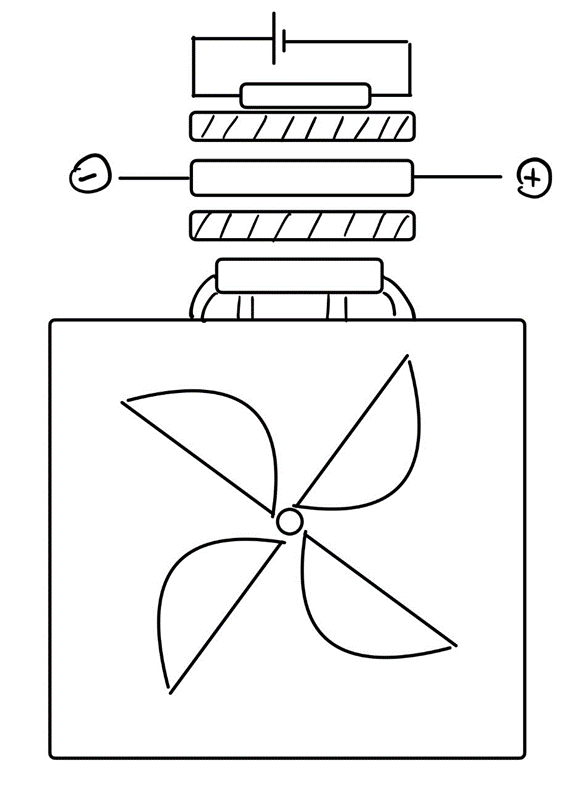
\includegraphics[width=0.45\textwidth]{热机示意图.png}
    %     \caption{热机示意图}
    %     \label{热机示意图}
    % \end{figure}


    % \begin{figure}[htbp]
    %     \centering
    %     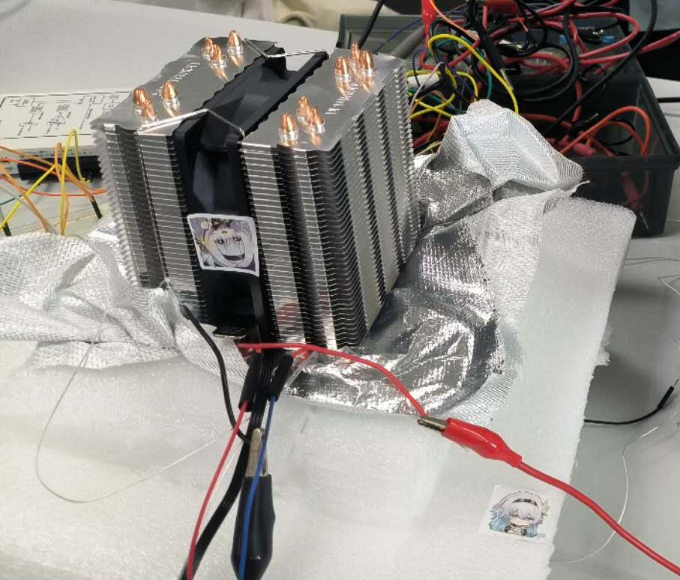
\includegraphics[width=0.45\textwidth]{热机实物图.png}
    %     \caption{热机实物图}
    %     \label{热机实物图}
    % \end{figure}

    \begin{figure}[htbp]
        \centering
        \subfloat[热机示意图]{%
            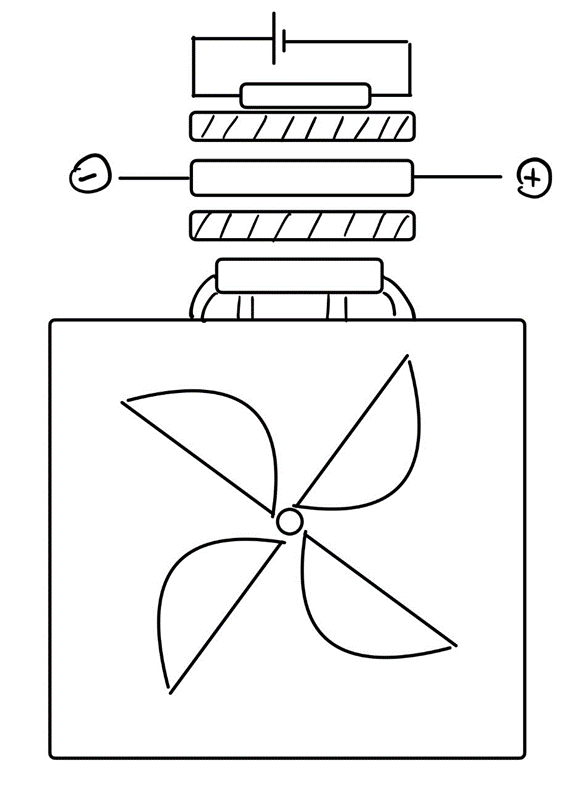
\includegraphics[width=0.31\textwidth]{热机示意图.png}
            \label{fig:热机示意图}
        }
        \quad
        \subfloat[热机实物图]{%
            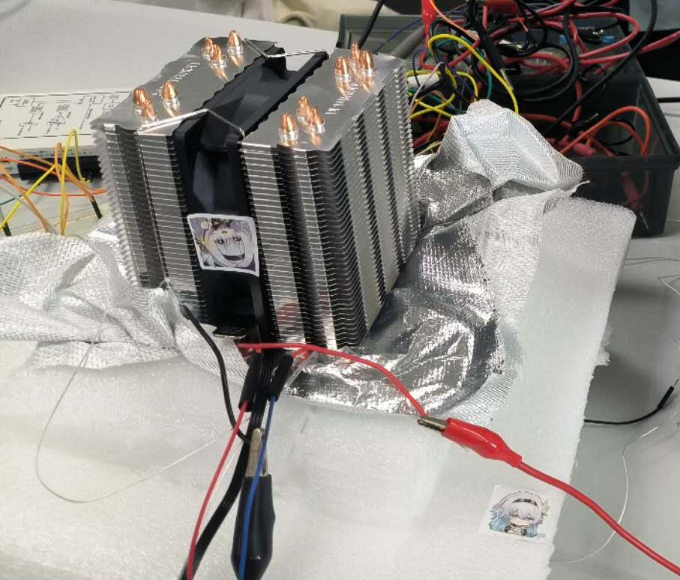
\includegraphics[width=0.31\textwidth]{热机实物图.png}
            \label{fig:热机实物图}
        }
        \caption{热机的示意图和实物图并排展示}
        \label{fig:热机}
    \end{figure}






\section{数据分析、误差讨论}









\section{总结及存在问题}












\end{document}
